\chapter{Tree Merge} \label{chap:merge}

Phylogenetic trees are essential to various evolutionary studies.
Due to their irreplaceable positions, many algorithms were
developed to reconstruct phylogenetic trees, including distance-based
methods\index{tree building algorithm!distance-based},
parsimony methods~\cite{fitch71}\index{tree building algorithm!parsimonious},
max-likelihood algorithms~\cite{felsenstein81}\index{tree building algorithm!maximum-likelihood}
and the recent Bayesian methods~\cite{rannala96}\index{tree building algorithm!Bayesian}.
Whereas these algorithms establish the fundament of
the theory of tree reconstruction, they have to work with certain
evolutionary models in practice such as
JTT~\cite{jones92}\index{JTT},
WAG~\cite{whelan01}\index{WAG},
HKY~\cite{hasegawa85}\index{HKY},
GY94~\cite{goldman94}\index{GY94}, and many more.
Given the variety of algorithms and models, is there an ultimate solution
to tree reconstruction problems? Unfortunately, the answer is `no'.
One of the major causes is the evolutionary heterogeneity over time.
Shifts in site-specific evolutionary rates, which is usually termed
as `heterotachy'\index{heterotachy}, frequently occur~\cite{lopez02}.
A model best fit one lineage or time frame may lead to erroneous inference
in another. Although this fact has already been noticed in several previous
works~\cite{weiss03,susko02} and extensively studied in the case
of few sequences~\cite{kolaczkowski04,gadagkar05,spencer05,philippe05},
little was achieved in solving the problem practically. Evolutionists
still have to build trees with
various algorithms and models, and combine the results with prior
knowledges and personal experiences. But how on earth do they
assess different trees? Is there a way to achieve this automatically?
This chapter aims to answer these two questions.

\begin{figure}[!hb]
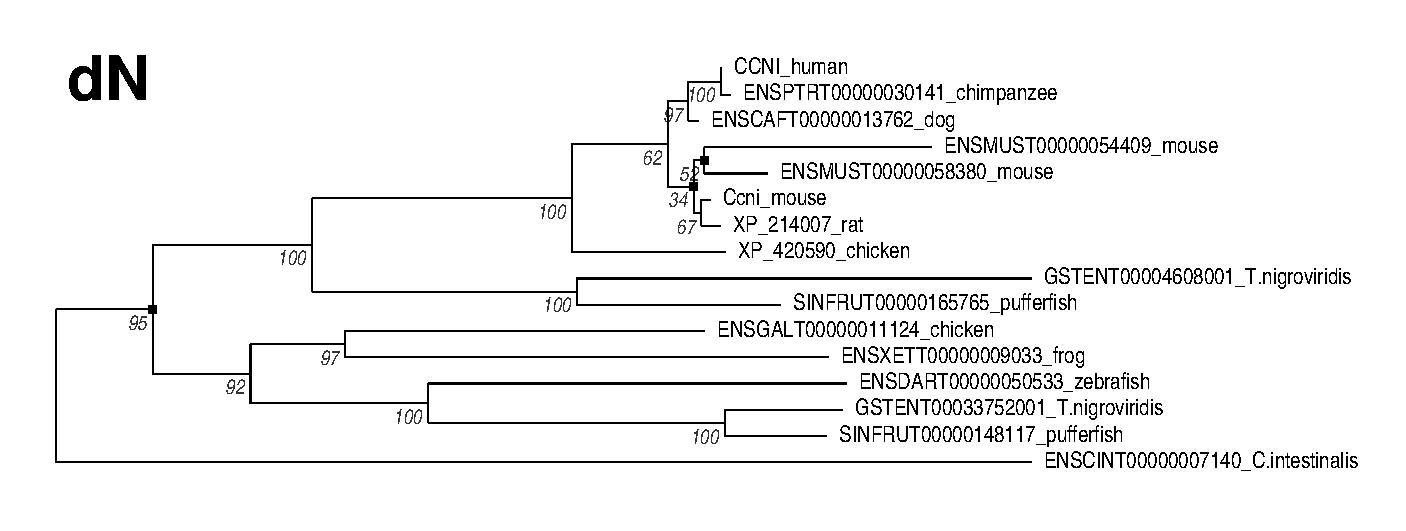
\includegraphics[width=\textwidth]{CCNI-dn}\\
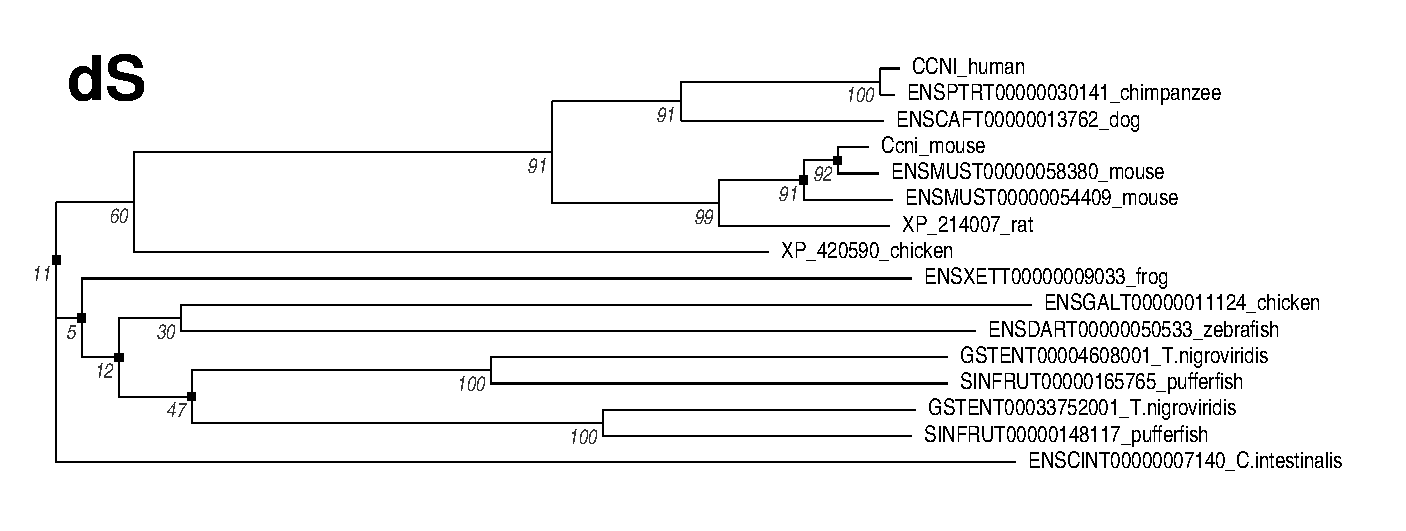
\includegraphics[width=\textwidth]{CCNI-ds}\\
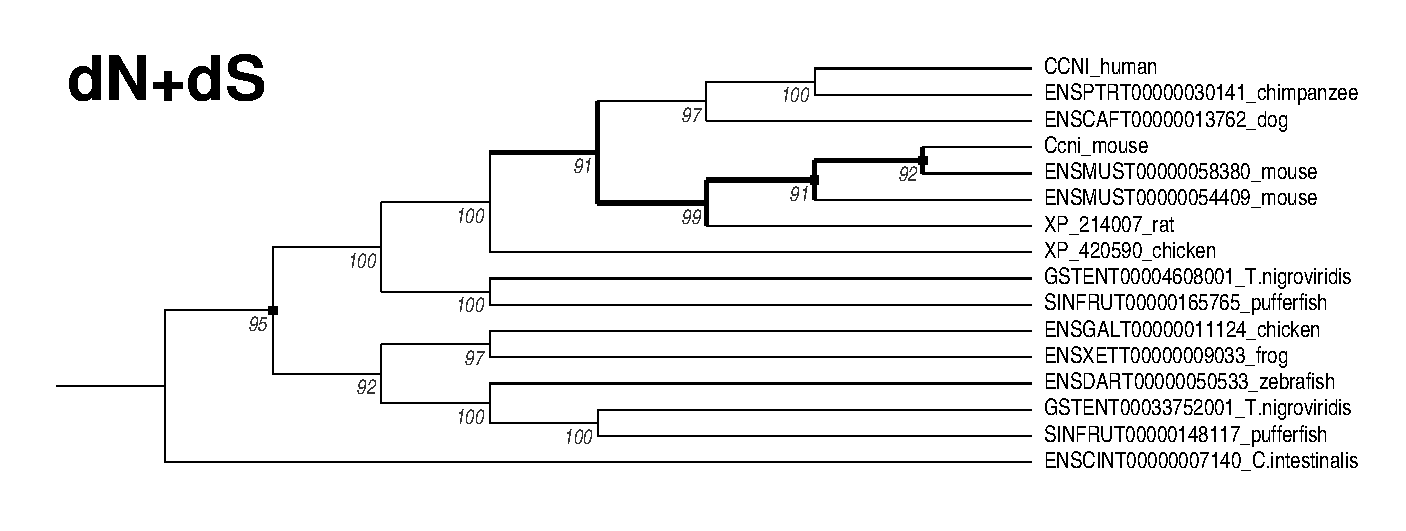
\includegraphics[width=\textwidth]{CCNI-dm}
\caption[Example of tree merge]{Example of tree merge. Non-synonymous tree {\bf dN}
	was merged with synonymous tree {\bf dS}, both reconstructed with neighbour-joining.
	Bold lines in the merged tree show the branches
	coming from {\bf dS}, while the rest from {\bf dN}. The resultant tree contains
	fewer losses and have higher bootstrapping support.	}\label{fig:mergeexam2}
\end{figure}

In order to understand how a tree can be evaluated by evolutionists,
let's first see an example. Figure~\ref{fig:mergeexam2} shows two trees reconstructed by neighbour-joining,
using synonymous distance ($d_s$) and non-synonymous
distance~\cite{nei86,li93,goldman94,yang00}\footnote{Nonsynonymous
distance ($d_n$) counts the number of nucleotide changes that contribute to
amino acid changes, while synonymous distance ($d_s$) counts the number that do not contribute to
amino acid changes.
Both kinds of distances can be only calculated in coding regions (CDS).
In theory, the synonymous distance $d_s$ tends to date the true evolutionary history more
precisely. Although selection for codon bias might occur, $d_s$ is generally less
influenced by heterogeneous selective pressure in different lineages~\cite{ayala99,baldauf03}.
However, if the two sequences are separated by a long evolutionary time, multiple
substitutions lead to saturation of $d_s$ and make it impossible to estimate $d_s$ accurately.
As a consequence, the deep branches of the $d_s$ tree are usually unreliable. Conversely, the
nonsynonymous distance $d_n$ is not saturated at long evolutionary time-frames and can
more effectively resolve the deep branches of the tree, but if the protein sequences are too similar,
too few non-synonymous changes will have accumulated to estimate $d_n$ accurately.
The lower branches of $d_n$ tree tend to be less accurate.} ($d_n$), respectively.
Even without any additional information, we can tell that the deeper branches
in $d_n$ tree and lower branches in $d_s$ tree are more likely to be correct.
This judgement is based on three rules: (i) reliable branches tend to
have higher bootstrapping support; (ii) synonymous trees are more effective
between close sequences, while nonsynonymous tree are better at deeper branches;
(iii) correct gene trees usually resemble the species tree.
If we can develop an algorithm that can account of these rules, it is possible
to automatically make a better tree by merging several trees built with different
methods. This is tree merge algorithm.

Tree merge is a process of choosing optimal
children between branches shared by candidate trees. As we want to shape the
algorithm in a precise and strict way, many abstract notations have to be used.
And therefore, we start this chapter by introducing the third type of representation of trees,
set representation. Then the tree merge problem is formally raised. After the description
and proof of the algorithm, we analyze the time complexity of this algorithm.
In the following chapter, the effectiveness of tree merge will be assessed together
with a lot of single-model algorithms.

\section{Set Representation of Trees}

Graph representation is more intuitive, but it is not convenient in comparing
rooted trees built from the same sequence set using different algorithms.
In graph language, identical trees are judged by comparing the
vertex sets and edge sets at the same time. But this is unnecessary. The edges or branches of a rooted
tree are naturally determined by the subset of leaves that are descendant from the lower node of the edge;
in turn, we can use a set of leaf subset to represent the topology of a rooted
tree~\footnote{Similarly, the topology of an unrooted tree can be represented as a set of
bipartitions of the leaf set}.
Thus, topological comparison can be reduced to set comparison, which is more
concise and straightforward.

\begin{figure}[!hb]
\begin{center}
\includegraphics{mpfig.10}
\caption[Example of set representation]
{Example of set representation. Set $\omega_G(g)$ is labeled at each internal node. The set representation
of $G$ is $\bar{G}=\{\{1\},\{2\},\{3\},\{4\},\{5\},\{2,3\},\{1,2,3\},\{1,2,3,4\},\{1,2,3,4,5\}\}$. Conversely,
when we get $\bar{G}$, we will also know the topology of $G$. Furthermore, if we let $\bar{g}=\{1,2,3\}$,
$\bar{G}|_{\bar{g}}=\{\{1\},\{2\},\{3\},\{2,3\},\{1,2,3\}\}$ is the set representation of $G|_g$.}\label{fig:example-set}
\end{center}
\end{figure}

Let $V$ be a leaf node set, and $\Sigma(V)=\{\mbox{$G$ is a rooted tree}:V_E(G)=V\}$ be the tree space in which each element
is a rooted tree whose external node set is $V$.
For any $G\in\Sigma(V)$, we can construct a set $\bar{G}\subset 2^V$~\footnote{Given a set $V$, $2^V=\{A:A\subset V\}$ is
the set of all the subsets of $V$ including $V$ itself and empty set $\emptyset$. $2^V$ is also called the $\sigma$-set of $V$.
Note that $\left|2^V\right|=2^{|V|}$ always stands. This is why it is written as $2^V$.}
using the $\omega_G$ map (Equation~\ref{equ:omega}) as follows:
\begin{equation}\label{equ:setrepre}
\bar{G}=\{\bar{g}\subset V:\bar{g}=\omega_G(g),g\in V(G)\}
\end{equation}
Obviously, $\bar{G_1}=\bar{G_2}$ only stands when the two trees $G_1$ and $G_2$ are topologically equivalent;
when $G_1$ differs $G_2$, $\bar{G_1}$ and $\bar{G_2}$ cannot be the same.
As a consequence, Equation~\ref{equ:setrepre} builds an one-to-one relation between
a set $\bar{G}$ and a graph $G$, and therefore $G$ can be represented by a set $\bar{G}$.
This is the set representation of a rooted tree.
When we know $\bar{G}$, we will always construct a tree $G$ under graph representation.
We also introduce:
\begin{equation}
\bar{G}|_{\bar{g}}=\{\bar{g}':\bar{g}'\in\bar{G}, \bar{g}'\subset\bar{g}\}
\end{equation}
Set $\bar{G}|_{\bar{g}}$ represents subtree $G|_g$. Figure~\ref{fig:example-set} shows an example.

Throughout this chapter, notations like $\bar{G}$ and $\bar{g}$ are always under the set representation.

\section{Set Forms of Duplication and Loss Functions}\label{sec:re-dl-fun}

In Section~\ref{sec:dl-fun}, the duplication and loss functions are defined as (Equation~\ref{equ:dl-fun}):
\begin{eqnarray}\label{equ:dl-fun-set}
D_G(g) &=& \left\{\begin{array}{ll}
    1 & \mbox{if $g$ is a duplication} \\
    0 & \mbox{otherwise}\end{array}\right. \\
L_G(g) &=& \sum_{g'\in\lhchild(g)}{|\lhloss(g')|}
\end{eqnarray}
The two functions defined in this way are dependent on the topology of the gene tree $G$.
As a matter of fact, if the parsimonious species map $M^*$ is applied to infer duplications and losses, the two functions
can be defined in a way independent of $G$. Let's re-examine the deduction of duplication and loss
under set representation.

In the following text, we always let $\bar{g}$, $\bar{g}_1$ and $\bar{g}_2$
be a subset of $V_E(G)$. From Equation~\ref{equ:par-M} and~\ref{equ:sigma}, we define:
\begin{eqnarray}
\sigma'(\bar{g}) &=& \{s_{g'}:g'\in \bar{g}\} \\
M^*(\bar{g}) &=& \lhlca(\sigma'(g)) \\
\sigma(\bar{g}) &=& \sigma'(g)\cup\left\{s\in V_E(S):\mbox{$\exists s'\in\sigma'(g)$, $\lhlca(s,s')<M^*(\bar{g})$}\right\}
\end{eqnarray}
Thus the parsimonious duplication function is:
\begin{equation}
D^*(\bar{g}_1,\bar{g}_2)=D^*(\bar{g}_2,\bar{g}_1)=\left\{\begin{array}{ll}
	1 & \mbox{if $\sigma(\bar{g}_1)\cap\sigma(\bar{g}_2)\not=\emptyset$;} \\
	0 & \mbox{otherwise.}\end{array}\right.
\end{equation}
Parsimonious loss function can be defined in a similar way:
\begin{equation}
L^*(\bar{g}_1,\bar{g}_2)=L^*(\bar{g}_2,\bar{g}_1)=|\lhloss^*(\bar{g}_1,\bar{g}_2)|+|\lhloss^*(\bar{g}_2,\bar{g}_1)|
\end{equation}
where
\begin{equation}
\lhloss'^*(\bar{g}_1,\bar{g}_2) = \left\{\begin{array}{ll}
	\sigma(\bar{g}_1\cup\bar{g}_2)\setminus\sigma(\bar{g}_1) & \mbox{if $D^*(\bar{g}_1,\bar{g}_2)=1$} \\
	\{s\in\sigma(\bar{g}_1\cup\bar{g}_2)\setminus\sigma(\bar{g}_1):\lhlca(s,M^*(\bar{g}_1))<M^*(\bar{g}_1\cup\bar{g}_2)\} & \mbox{otherwise}
\end{array}\right.
\end{equation}
\begin{equation}
\lhloss^*(\bar{g}_1,\bar{g}_2) = \{s\in V(S):\omega_S(s)\subset\lhloss'(\bar{g}_1,\bar{g}_2),\omega_S(\lhparent(s))\not\subset\lhloss'(\bar{g}_1,\bar{g}_2)\}
\end{equation}
They correspond to Equation~\ref{equ:loss1} and~\ref{equ:loss2}.
Now, parsimonious duplication and loss functions can be calculated given two set of leaves.
Such calculation is topology-independent in the sense that the topologies on the two sets
will not affect the calculation process. This property is particularly useful
in constructing the objective function for tree merge algorithm~\ref{sec:merge-obj-fun}.

\section{Tree Merge}

\subsection{Tree merge problem}

Given a set of \emph{binary rooted} trees $\Phi=\{\bar{G}_1,\bar{G}_2,\ldots,\bar{G}_n\}$, define a permitted branch set:
\begin{equation}
\mathcal{G}(\Phi)=\bigcup_{\bar{G}'\in\Phi} \bar{G'}
\end{equation}
Let $\Omega(\mathcal{G})$ be the set of binary rooted tree $\bar{G}$ that satisfies $\bar{G}\subset\mathcal{G}$.
Being a subset of $\Sigma(V)$, $\Omega(\mathcal{G})$
is the tree space spanned by $\bar{G}_1,\bar{G}_2,\ldots,\bar{G}_n$.
It is also useful to define a permitted branch set $\mathcal{G}|_{\bar{g}}$ that
is restricted to a node $\bar{g}$:
\begin{equation}
\mathcal{G}|_{\bar{g}} = \bigcup_{\bar{G}'\in\Phi} \bar{G}'|_{\bar{g}}
\end{equation}
Then $\Omega(\mathcal{G}|_{\bar{g}})$ is the tree space spanned by $\bar{G}_1|_{\bar{g}},\bar{G}_2|_{\bar{g}},\ldots,
\bar{G}_n|_{\bar{g}}$.

Let $F$ be a function defined on $\Sigma(V)$. The \emph{general tree merge problem}
\index{tree merge problem!general tree merge problem} is to find a \emph{binary rooted} tree
$\bar{G}\in\Omega(\mathcal{G})$ that optimizes $F(\cdot)$. For common $F$, the only solution is to
enumerate every tree in $\Omega$ and then search for the optimum one. But for
a class of special objective functions, the exhaustive search can be replaced by a simple precise
algorithm. In this thesis, we only consider functions that take the form:
\begin{equation}\label{equ:independent}
F(\bar{G})=\sum_{\bar{g}\in \bar{G}}f(\lhchild(\bar{g}))=\sum_{\bar{g}\in \bar{G}}f(\bar{g}_1,\bar{g}_2)
\end{equation}
Such an $F(\bar{G})$ has two critical properties. First, it is additive, and second,
function $f$ is defined on $2^V\times 2^V$, which means that the calculation of $f(\lhchild(\bar{g}))$ is
only dependent on the elements in $\bar{g}$'s children set but independent of the topologies of
$\bar{g}$'s children. As we will see in the following section,
these two properties, especially the second one, guarantee that the optimum tree can be
found in $O(|\Phi|\cdot|V|^2)$ time.
The (special) \emph{tree merge problem}\index{tree merge problem} is to find the optimal \emph{binary rooted} tree
in $\Omega(\mathcal{G})$ when $F(\bar{G})$ follows Equation~\ref{equ:independent}.

\subsection{Constructing objective functions}\label{sec:merge-obj-fun}

According to Equation~\ref{equ:independent}, the effectiveness of tree merge algorithm
totally relies on function $f$. Before detailed algorithm is described, we should make
sure that $f$ is present and biologically reasonable.

Based on the discussion in Section~\ref{sec:re-dl-fun}, $f$ can be defined as:
\begin{equation}\label{equ:f-obj}
f(\bar{g}_1,\bar{g}_2)=f(\bar{g}_2,\bar{g}_1)=\alpha D^*(\bar{g}_1,\bar{g}_2)
	+\beta L^*(\bar{g}_1,\bar{g}_2)-\gamma B^*(\bar{g}_1,\bar{g}_2)
\end{equation}
where $\alpha,\beta,\gamma>0$, $D^*(\bar{g}_1,\bar{g}_2)$ and $L^*(\bar{g}_1,\bar{g}_2)$ are
the duplication and losses functions, respectively, and $B^*(\bar{g}_1,\bar{g}_2)$ denotes
the highest bootstrapping supports among all trees containing $\{\bar{g}_1,\bar{g}_2\}$.
Note that the star in in $D^*$ and $L^*$ indicates the parsimonious species map
$M^*$ is used in DLI inference. These two functions measure the similarity between
a gene tree and the species tree. The smaller, the better.
As to $B^*(\bar{g}_1,\bar{g}_2)$, another possible
definition is also available, which will be discussed in the end of this chapter.
%However, when the majority of candidates
%are built from similar algorithms, such a $B^*$ will favour
%them because similar algorithms tend to result in similar topologies.
%And therefore the previous definition is more appropriate.
In addition, if we know
that certain algorithm is good at particular branches, we can deliberately
raise the bootstrapping supports. Consequently, all the three rules addressed in
the introduction section of this chapter have been considered.

\subsection{Tree merge algorithm}

The basic idea of tree merge algorithm resembles that of dynamic programming. It reduces
exhaustive search to the calculation of a function $F^*(\bar{g})$ for each $\bar{g}\in\mathcal{G}$.
$F^*$ is defined as:
\begin{equation}\label{equ:F-star}
F^*(\bar{g}) = \min_{\bar{G}|_{\bar{g}}\in\Omega(\mathcal{G}|_{\bar{g}})} F(\bar{G}|_{g})
\end{equation}
Obviously, $F^*(V) = \min F(\bar{G})$ always stands. Thus searching optimal tree $\bar{G}$
is equivalent to calculating $F^*(V)$. When $F(\cdot)$ follows Equation~\ref{equ:independent},
$F^*(V)$ can be calculated recursively. To achieve this goal, we need to construct
the set of permitted children pairs given a node $\bar{g}$:
\begin{equation}\label{equ:C-set}
\mathcal{C}(\bar{g}) = \left\{\{\bar{g}_1,\bar{g}_2\}:\mbox{$\bar{g}_1,\bar{g}_2\in\mathcal{G}$, $\bar{g}_1\cap\bar{g}_2=\emptyset$ and $\bar{g}_1\cup\bar{g}_2=\bar{g}$}\right\}
\end{equation}
Set $\mathcal{C}(\bar{g})$ consists of $\bar{g}$'s candidate children set. That is,
each element $\{\bar{g}_1,\bar{g}_2\}\in\mathcal{C}(\bar{g})$ can be $\bar{g}$'s children set. Then,
\begin{eqnarray*}
&&F^*(\bar{g})\\
&=& \min_{\bar{G}|_{\bar{g}}\in\Omega(\mathcal{G}|_{\bar{g}})} F(\bar{G}|_{g})\\
&=& \min_{\bar{G}|_{\bar{g}}\in\Omega(\mathcal{G}|_{\bar{g}})}\sum_{\bar{g}'\in \bar{G}|_{\bar{g}}}f(\lhchild(\bar{g}')) \\
&=& \min_{\{\bar{g}_1,\bar{g}_2\}\in\mathcal{C}(\bar{g})}\left\{
	\min_{\bar{G}|_{\bar{g}_1}\in\Omega(\mathcal{G}|_{\bar{g}_1})}\sum_{\bar{g}'_1\in \bar{G}|_{\bar{g}_1}}f(\lhchild(\bar{g}'_1))
	+ f(\bar{g}_1,\bar{g}_2)
	+ \min_{\bar{G}|_{\bar{g}_2}\in\Omega(\mathcal{G}|_{\bar{g}_2})}\sum_{\bar{g}'_2\in \bar{G}|_{\bar{g}_2}}f(\lhchild(\bar{g}'_2))\right\}
\end{eqnarray*}
From Equation~\ref{equ:F-star} and~\ref{equ:independent}, we know that:
\begin{equation}\label{equ:cal-F-star}
F^*(\bar{g}) = \min_{\{\bar{g}_1,\bar{g}_2\}\in\mathcal{C}(\bar{g})}\left\{F^*(\bar{g}_1)+f(\bar{g}_1,\bar{g}_2)+F^*(\bar{g}_2)\right\}
\end{equation}
Thus $F^*(V)$ can be calculated recursively.

\begin{table}[!hb]
\begin{center}
\begin{tabular}{|l|}
\hline
{\bf Function:}\\
\lhspace{\sc TreeMerge}$(V,\bar{G}_1,\bar{G}_2,\ldots,\bar{G}_n)$\\
{\bf Input:} \\
\lhspace$n$ gene trees $\bar{G}_1,\bar{G}_2,\ldots,\bar{G}_n\in\Sigma(V)$; \\
{\bf Output:} \\
\lhspace Tree $\bar{G}^*$ by merging $\bar{G}_1,\bar{G}_2,\ldots,\bar{G}_n$\\
{\bf Procedures:} \\
\lhspace$\mathcal{G}\leftarrow\emptyset$ \\
\lhspace$\mathcal{C}\leftarrow\emptyset$ \\
\lhspace{\sc ConstructG}$(\bar{G}_1,\ldots,\bar{G}_n)$ \\
\lhspace\lhspace{\bf for} $i = 1$ {\bf to} $n$ {\bf do} \\
\lhspace\lhspace\lhspace{\bf for} each $\bar{g}\in \bar{G}_i$ {\bf do} \\
\lhspace\lhspace\lhspace\lhspace$\mathcal{G}\leftarrow\mathcal{G}\cup\{\bar{g}\}$ \\
\lhspace\lhspace\lhspace\lhspace$\mathcal{C}(\bar{g})\leftarrow\mathcal{C}(\bar{g})\cup\{\lhchild(\bar{g})\}$ \\
\\
\lhspace$selected\gets\emptyset$\\
\lhspace{\sc OptimizeF}$(\bar{g})$ \\
\lhspace\lhspace{\bf if} $F^*(\bar{g})$ has been calculated {\bf then} \\
\lhspace\lhspace\lhspace{\bf return} $F^*(\bar{g})$ \\
\lhspace\lhspace$min\leftarrow\infty$ \\
\lhspace\lhspace{\bf for} each $\{\bar{g}_1,\bar{g}_2\}\in\mathcal{C}(\bar{g})$ {\bf do} \\
\lhspace\lhspace\lhspace$score\gets\mbox{{\sc OptimizeF}}(\bar{g}_1)+f(\bar{g}_1,\bar{g}_2)+\mbox{{\sc OptimizeF}}(\bar{g}_2)$\\
\lhspace\lhspace\lhspace{\bf if} $min>score$ {\bf then}\\
\lhspace\lhspace\lhspace\lhspace$min\gets score$\\
\lhspace\lhspace\lhspace\lhspace$minpair\gets \{\bar{g}_1,\bar{g}_2\}$\\
\lhspace\lhspace$F^*(\bar{g})\gets min$ \\
\lhspace\lhspace$selected(\bar{g})\gets minpair$ \\
\\
\lhspace{\sc BuildTree}$(\bar{g})$ \\
\lhspace\lhspace{\bf if} $selected(\bar{g})=\emptyset$ {\bf then}\\
\lhspace\lhspace\lhspace{\bf return} $\{\bar{g}\}$\\
\lhspace\lhspace$\{\bar{g}_1,\bar{g}_2\}\gets selected(\bar{g})$\\
\lhspace\lhspace{\bf return} $\mbox{\sc BuildTree}(\bar{g}_1)\cup\{\bar{g}\}\cup\mbox{\sc BuildTree}(\bar{g}_2)$\\
\\
\lhspace{\sc TreeMerge}$(V,\bar{G}_1,\bar{G}_2,\ldots,\bar{G}_n)$\\
\lhspace\lhspace{\sc ConstructG}$(\bar{G}_1,\ldots,\bar{G}_n)$\\
\lhspace\lhspace{\bf for} each $v\in V$ {\bf do}\\
\lhspace\lhspace\lhspace$F^*(\{v\})\gets 0$\\
\lhspace\lhspace{\sc OptimizeF}$(V)$\\
\lhspace\lhspace{\bf return} {\sc BuildTree}$(V)$\\
\hline
\end{tabular}
\caption[Tree merge algorithm]
{Tree merge algorithm. Procedure {\sc ConstructG} constructs $\mathcal{G}$ and $\mathcal{C}(\bar{g})$;
{\sc OptimizeF} recursively calculates $F^*(\bar{g})$ and stores optimum children
in $selected$, from which {\sc BuildTree} builds the merge tree. {\sc BuildTree}
generates a tree in set presentation. It can also be easily adapted to generate a tree
$G^*=(V(G^*),E(G^*))$ in graph presentation.}~\label{tab:merge}
\end{center}
\end{table}

\begin{figure}[!hb]
\begin{center}
\includegraphics{mpfig.7}
\caption[Example of tree merge algorithm]{Example of tree merge algorithm. Tree $G_1$ and $G_2$ are
merged into $G^*$. Bold nodes show the duplications and the number beside a branch is
the number of losses occuring at that branch. For example, $|\lhloss(\{mou_1\},\bar{g}_3)|=|\{{\it Rat}\}|=1$
and $|\lhloss(\bar{g}_1^c,\bar{g}_6)|=|\{{\it Human, Chicken}\}|=2$.}\label{fig:merge-exa}
\end{center}
\end{figure}

The two equations, \ref{equ:C-set} and \ref{equ:cal-F-star}, established the basis of tree merge algorithm. Table~\ref{tab:merge}
presents more details. In practical implementation, hash technique should be applied
to judge whether $\bar{g}$ has been inserted to $\mathcal{G}$. If the hash function
is perfect, only $O(|V|)$ time is needed to locate and insert a set to $\mathcal{G}$.
This will greatly accelerate the algorithm.

Hash technique makes tree merge very efficient. In procedure {\sc ConstructG}, all the hash values can be
calculated in $O(n\cdot|V|(|V|-1))$. The following $n\cdot(|V|-1)$ times of set comparisons and insertions
take $O(n\cdot|V|^2)$ time at most. Procedure
{\sc OptimizeF} traverses all possible $\bar{g}\in\mathcal{G}$ and $\bar{g}$'s bipartition
$\bar{g}=\bar{g}_1\cup\bar{g}_2$. The time complexity in this part is also $O(n\cdot|V|^2)$.
Both {\sc BuildTree} and {\sc TreeMerge} can be achieved in $O(|V|)$. Consequently, the time complexity
of tree merge is $O(n\cdot|V|^2)$.

Figure~\ref{fig:merge-exa} gives an example of tree merge process.
In this example, $\mathcal{G}=\{\{hum\},\{mou_1\},\{mou_2\},\{rat\},\{chi\},\bar{g}^c_1,
\bar{g}^c_2,\bar{g}_3,\bar{g}_4,\bar{g}_5,\bar{g}_6\}$,
$\mathcal{C}(\bar{g}^c_1)=\left\{\{\bar{g}_3,\{mou_2\}\},\{\{rat\},\bar{g}_5\}\right\}$
and $\mathcal{C}(\bar{g}^c_2)=\left\{\{\bar{g}_4,\{chi\}\},\{\bar{g}^c_1,\bar{g}_6\}\right\}$.
Only $\mathcal{C}(\bar{g}^c_1)$ and $\mathcal{C}(\bar{g}^c_2)$ consist of more than one node pairs. Other $\mathcal{C}(\cdot)$ just
has one element. If we let $\alpha=\beta=1$ and $\gamma=0$ in Euqation~\ref{equ:f-obj},
we know that $f(\bar{g}_3,\{mou_2\})=1+1=2$, $f(\{rat\},\bar{g}_5)=0$, $F^*(\bar{g}_5)=1$ and $F^*(\bar{g}_3)=0$. Thus
$F^*(\bar{g}^c_1)=\min\{0+2+0,0+0+1\}=1$. The children pair $\{\{rat\},\bar{g}_5\}$ is preferable.
Similarly, as $f(\bar{g}_4,\{chi\})=0$, $f(\bar{g}^c_1,\bar{g}_6)=3$, $F^*(\bar{g}_4)=1+0+0=1$
and $F^*(\bar{g}_6)=1$, $F^*(\bar{g}^c_2)=\min\{1+0+0,1+3+1\}=1$.
The children pair $\{\bar{g}_4,\{chi\}\}$ is preferred. Consequently,
$\bar{G}^*=\{\{hum\},\{mou_1\},\{mou_2\},\{rat\},\{chi\},\bar{g}_1^c,\bar{g}_2^c,\bar{g}_4\}$ gives the final tree
and $F(G^*)=F^*(\bar{g}^c_2)=1$.

\section{Discussions}
Tree merge is able to capture the thinking of evolutionists. Although not
a tree-building algorithm by itself, tree merge can combine the advantages of
different tree-building algorithms and models, and automatically choose suitable
methods in different lineages. It is most useful when candidate trees
can compensate for the deficiency of one another. However,
just as evolutionists cannot reconstruct correct trees
without reasonable candidate trees, tree merge is less useful or even wrong
if artefact candidates are provided. Sometimes a human being can detect the artefacts
and make a tree outside $\Omega$ tree space, but tree merge cannot achieve.
This is the theoretical limitation. Furthermore, the performance of tree merge is
determined by the objective function. An evolutionary history that breaks
the optimization process will fail tree merge, either.
When using tree merge algorithm, we should pay attention to these points.

Tree merge algorithm can also be considered as an alternative algorithm to make
a consensus tree~\cite{margush81} from a set of resampled trees. All we need is to modify the definition of $B^*(\bar{g}_1,\bar{g}_2)$
in Equation~\ref{equ:f-obj}. Assume we have $n$ resampled binary rooted gene trees $\Phi=\{\bar{G}_1,\bar{G}_2,\ldots,\bar{G}_n\}$.
Given $\bar{g}_1,\bar{g}_2\in\mathcal{G}(\Phi)$, we can define $B^*(\bar{g}_1,\bar{g}_2)$ as the number of times when
$\{\bar{g}_1\cup\bar{g}_2\}\subset\bar{G}_i$, $i=1,\ldots,n$\footnote{$B^*$
can also be defined in other similar, but different, ways.}. In this way,
$B^*(\bar{g}_1,\bar{g}_2)$ is the bootstrapping supports for a branch $\{\bar{g}_1,\bar{g}_2\}$.
And if we set $\alpha=\beta=0$, tree merge process is actually the same as that of making a consensus tree from a set of
binary rooted trees. In conclusion, when $B^*$ is defined as above, tree merge extends (rooted) consensus
tree algorithms by incorporating species evolution, and may help to improve the quality of the consensus tree.

Tree merge is designed to work with a binary rooted gene tree where the phylogeny
of species is clear. How to root a tree was discussed in~\ref{chap:buildtree}.
In principle, it is also possible to extend the algorithm in case of unrooted trees,
but most of concepts in this chapter should be modified accordingly.
Resolving a multifurcated tree is also tactable. Durand {\it et al.}~\cite{durand06} implies
an algorithm that may be adapted to resolve polytomies by minimizing duplications and losses.
In contrast, the requirement of species phylogeny is critical. To our experience, no other criterion that
satisfies Equation~\ref{equ:independent} can be as effective as this standard.
